\begin{song}{title=\predtitle \centering John Brown's body \\\large  }  %% sem se napíše jméno songu a autor


\vspace*{-0.43cm}
\vetsi

\moveleft 0.6cm \vbox{

\begin{centerjustified}
\begin{varwidth}[t]{0.5\textwidth}\setlength{\parindent}{\pindent}  %Varianta č. 2 --> Dva sloupce

\vspace*{-0.43cm}


\sloka
^{G\z}John Brown’s body lies moldering in

the grave,

While ^{C\z}weep the sons of bondage whom

he ^{G\z}ventured all to save;

But tho he lost his life while struggling

for the ^{Emi}slave,

His ^{A7}soul is ^{D7\z}marching ^{G}on.

\refren
^{G\z}Glory, glory, hallelujah!

^{C\z}Glory, glory, ^{G}hallelujah!

Glory, glory, ^{\z Emi}hallelujah!

^{Ami\z }his~soul's ^{D7\z}marching ^{G}on!

\sloka
John Brown was a hero, undaunted,

true and brave,

And Kansas knows his valor when he

fought her rights to save;

Now, tho the grass grows green above

his grave,

His soul is marching on.

\refren

\sloka
He captured Harper’s Ferry, with his

nineteen men so few,

And frightened Old Virginny till she

trembled thru and thru;

They hung him for a traitor,

themselves the traitor crew,

But his soul is marching on.

\refren



\end{varwidth}\begin{varwidth}[t]{0.55\textwidth}\setlength{\parindent}{\pindent}
\vspace*{0.03cm}


\sloka
John Brown was John the Baptist of the

Christ we are to see,

Christ who of the bondmen shall the

Liberator be,

And soon throug the Sunny South the

slaves shall all be free,

For his soul is marching on.

\refren


\sloka
The conflict that he heralded he looks from

heaven to view,

On the army of the Union with its flag red,

white and blue.

And heaven shall ring with anthems o’er

the deed they mean to do,

For his soul is marching on.

\refren

\sloka
Ye soldiers of Freedom, then strike, while

strike ye may,

The death blow of oppression in a better

time and way,

For the dawn of old John Brown has

brightened into day,

And his soul is marching on.

\refren

\hrulefill

\vspace*{.1cm}

\begin{varwidth}{.5\textwidth}
Otroctví bylo v USA zakázáno r. 1865.

I~dnes otroctví v~jistých částech světa přetrvává.
%např. firma
%Nestlé prý používá dětské otroky.

Afroameričané však stále v~USA čelí systémovému rasismu.
Např. r. 2022 je v tamních vězeních celkem 2 miliony lidí, z toho 38 \% afr., i
když tvoří jen 12 \% populace.
\end{varwidth}
\begin{varwidth}{.2\textwidth}
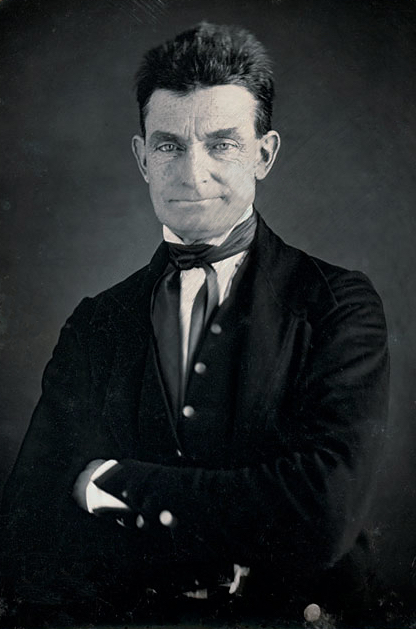
\includegraphics[width=4cm]{../img/JohnBrown.jpg}
\end{varwidth}



\end{varwidth}
\end{centerjustified}


}




\setcounter{Slokočet}{0}
\end{song}

